
\chapter{Advanced Derivatives}
\label{chapter:advanced}

In the Simple Derivatives chapter every network was built purely from contractions,
so differentiation was just ``delete the node''.
The remaining derivatives of the Matrix Cookbook involve a few genuinely nonlinear atoms:
inverses, determinants, eigenvalues, norms, and structural constraints.
The pleasant surprise is that each atom needs exactly \emph{one} new local rule,
and after applying it, delete-the-node does the rest.

\section{Derivatives of an Inverse}

Differentiating both sides of $X^{-1} X = I$ with the product rule gives
$\mathrm{d}(X^{-1}) X + X^{-1} \mathrm{d}X = 0$, so
$\mathrm{d}(X^{-1}) = -X^{-1}\, \mathrm{d}X\, X^{-1}$.
In diagrams this is a \emph{splitting rule}: to differentiate through an inverse node,
split it into two inverse nodes with the new derivative edges dangling in between,
and flip the sign:
\[
   \begin{tikzpicture}[baseline=(a0.base), inner sep=1pt]
      \node (a0) {$(X^{-1})$};
      \draw (a0.west) -- ++(-.4,0);
      \draw (a0.east) -- ++(.4,0);
      \draw[d] (a0.north east) -- ++(.2,.2);
      \draw[d] (a0.north east) -- ++(.3,.1);
   \end{tikzpicture}
   \;=\;
   -\;
   \begin{tikzpicture}[baseline=(b0.base), inner sep=1pt]
      \node (b0) {$X^{-1}$};
      \node[right=1.2em of b0] (b1) {$X^{-1}$};
      \draw (b0.west) -- ++(-.4,0);
      \draw (b0.east) -- ++(.3,.15);
      \draw (b1.west) -- ++(-.3,.15);
      \draw (b1.east) -- ++(.4,0);
   \end{tikzpicture}
\]
Note the rule contains the plain matrix case:
if $X^{-1}$ appears once in any network, its derivative replaces the node by the split pair.
The Matrix Cookbook's versions:
\begin{walign}
   \tag{59}
   \frac{\partial Y^{-1}}{\partial x}
   &= -Y^{-1}\frac{\partial Y}{\partial x} Y^{-1}
   \\
   \tag{61}
   \frac{\partial a^T X^{-1} b}{\partial X}
   &= -X^{-T} a b^T X^{-T}
   &
   \begin{tikzpicture}[baseline=(a0.base), inner sep=1pt]
      \node (a0) {$(a$};
      \node[right=.7em of a0] (a1) {$X^{-1}$};
      \node[right=.7em of a1] (a2) {$b)$};
      \draw (a0) -- (a1) -- (a2);
      \draw[d] (a2.east) -- ++(.2,.2);
      \draw[d] (a2.east) -- ++(.3,.1);
   \end{tikzpicture}
   &=
   -\,
   \begin{tikzpicture}[baseline=(a0.base), inner sep=1pt]
      \node (a0) {$a$};
      \node[right=.6em of a0] (a1) {$X^{-1}$};
      \node[right=1.4em of a1] (a2) {$X^{-1}$};
      \node[right=.6em of a2] (a3) {$b$};
      \draw (a0) -- (a1);
      \draw (a1.east) -- ++(.3,.15);
      \draw (a2.west) -- ++(-.3,.15);
      \draw (a2) -- (a3);
   \end{tikzpicture}
   \\
   \tag{63}
   \frac{\partial \Tr(A X^{-1} B)}{\partial X}
   &= -(X^{-1} B A X^{-1})^T
   &
   \begin{tikzpicture}[baseline=(a0.base), inner sep=1pt]
      \node (a0) {$(A$};
      \node[right=.7em of a0] (a1) {$X^{-1}$};
      \node[right=.7em of a1] (a2) {$B)$};
      \draw (a0) -- (a1) -- (a2);
      \path (a0) edge [out=155, in=25, looseness=1.5] (a2);
      \draw[d] (a2.south east) -- ++(.2,-.2);
      \draw[d] (a2.south east) -- ++(.3,-.1);
   \end{tikzpicture}
   &=
   -\,
   \begin{tikzpicture}[baseline=(a0.base), inner sep=1pt]
      \node (a0) {$X^{-1}$};
      \node[right=.6em of a0] (a1) {$B$};
      \node[right=.6em of a1] (a2) {$A$};
      \node[right=.6em of a2] (a3) {$X^{-1}$};
      \draw (a0) -- (a1) -- (a2) -- (a3);
      \draw (a0.west) -- ++(-.3,.15);
      \draw (a3.east) -- ++(.3,.15);
   \end{tikzpicture}
   \\
   \tag{64}
   \frac{\partial \Tr((X+A)^{-1})}{\partial X}
   &= -\big((X+A)^{-1}(X+A)^{-1}\big)^T
\end{walign}
In (61) and (63) we simply split the inverse node;
the two dangling stubs are the row and column of the result,
and reading them off gives the classical transposes.
In (63), the trace loop connects the two split halves into the single chain
$X^{-1} B A X^{-1}$.

When the inverse's \emph{argument} contains $X$ several times, the product rule adds one
split term per occurrence.
For $B$ and $C$ symmetric the Matrix Cookbook lists
\begin{walign}
   \tag{125}
   &\frac{\partial}{\partial X} \Tr\big[(X^T C X)^{-1} A\big]
   \\*
   &= -\big(CX (X^T C X)^{-1}\big)(A + A^T)(X^T C X)^{-1}
   \\
   \tag{126}
   &\frac{\partial}{\partial X} \Tr\big[(X^T C X)^{-1} (X^T B X)\big]
   \\*
   &= -2 C X (X^T C X)^{-1} X^T B X (X^T C X)^{-1}
   + 2 B X (X^T C X)^{-1}
   \\
   \tag{127}
   &\frac{\partial}{\partial X} \Tr\big[(A + X^T C X)^{-1} (X^T B X)\big]
   \\*
   &= -2 C X (A + X^T C X)^{-1} X^T B X (A + X^T C X)^{-1}
   + 2 B X (A + X^T C X)^{-1}
\end{walign}
These all follow mechanically:
delete the two $X$'s of the inner $X^T B X$ (the $+2BX(\cdots)^{-1}$ terms),
and split the inverse around the two $X$'s inside it (the $-2CX(\cdots)$ terms);
the factors of $2$ come from the symmetry of $B$ and $C$ pairing up the terms.
We leave the diagram derivation of (126) as an exercise.

\section{Derivatives of a Determinant}

Recall from the previous chapter that $\det(X)$ is the closed diagram
of $n$ copies of $X$ between two (normalized) anti-symmetrizer bars.
The node $X$ appears $n$ times,
so delete-the-node gives a sum of $n$ networks with one copy removed ---
and by the symmetry of the bars, all $n$ are equal:
\[
   \frac{\partial \det(X)}{\partial X}
   \;=\;
   n\,\cdot
   \mathbin{\begin{tikzpicture}[baseline=(a0.base), inner sep=1pt]
      \node (a0) {$X$};
      \node[right=.5em of a0] (dots) {$\cdots$};
      \node[right=.5em of dots] (a1) {$X$};
      \node[right=1em of a1] (g) {\phantom{$X$}};
      \draw (a0.north) -- ++(0,.2) coordinate (a0top);
      \draw (a1.north) -- ++(0,.2) coordinate (a1top);
      \draw (a0.south) -- ++(0,-.2) coordinate (a0bot);
      \draw (a1.south) -- ++(0,-.2) coordinate (a1bot);
      \draw (g.north) ++(0,.2) coordinate (gtop) -- ++(0,-.15);
      \draw (g.south) ++(0,-.2) coordinate (gbot) -- ++(0,.15);
      \draw[line width=2pt] (a0top -| a0.west) -- (gtop -| g.east);
      \draw[line width=2pt] (a0bot -| a0.west) -- (gbot -| g.east);
   \end{tikzpicture}}
\]
The diagram on the right --- $n-1$ copies of $X$ with one empty slot ---
is a matrix in the two dangling edges.
Classically it is $\frac{1}{n}\operatorname{adj}(X)^T$, the (transposed, scaled) \emph{adjugate},
and for invertible $X$ it equals $\frac1n \det(X)\, X^{-T}$.
So we recover the Matrix Cookbook identities
\begin{walign}
   \tag{49}
   \frac{\partial \det(X)}{\partial X}
   &= \det(X)\, (X^{-1})^T
   \\
   \tag{46}
   \frac{\partial \det(Y)}{\partial x}
   &= \det(Y) \Tr\Big[Y^{-1} \frac{\partial Y}{\partial x}\Big]
   \\
   \tag{57}
   \frac{\partial \ln|\det(X)|}{\partial X}
   &= (X^{-1})^T
   \\
   \tag{51}
   \frac{\partial \det(AXB)}{\partial X}
   &= \det(AXB)\, (X^{-1})^T
   \\
   \tag{58}
   \frac{\partial \det(X^k)}{\partial X}
   &= k \det(X^k)\, X^{-T}
\end{walign}
where (46) is the chain-rule form of (49),
(57) follows since $\mathrm{d}\ln\det = \mathrm{d}\det/\det$,
and (51), (58) are exercises
(in (58) the closed stack contains $kn$ copies of $X$).

\subsection{The Characteristic Polynomial}
The determinant of $I + tA$ collects the \emph{elementary symmetric polynomials}
$e_k$ of the eigenvalues of $A$,
and each has a clean diagram:
$e_k$ is the closed stack of just $k$ copies of $A$ between bars of width $k$.
\[
   \det(I + tA) = \sum_{k=0}^{n} t^k e_k,
   \qquad
   e_1 = \trace{A}{2}\,,
   \qquad
   e_2 =
   \mathbin{\begin{tikzpicture}[baseline=(a0.base), inner sep=1pt]
      \node (a0) {$A$};
      \node[right=1em of a0] (a1) {$A$};
      \draw (a0.north) -- ++(0,.2) coordinate (a0top);
      \draw (a1.north) -- ++(0,.2) coordinate (a1top);
      \draw (a0.south) -- ++(0,-.2) coordinate (a0bot);
      \draw (a1.south) -- ++(0,-.2) coordinate (a1bot);
      \draw[line width=2pt] (a0top -| a0.west) -- (a1top -| a1.east);
      \draw[line width=2pt] (a0bot -| a0.west) -- (a1bot -| a1.east);
   \end{tikzpicture}}
   \;=\; \tfrac12\big(\Tr(A)^2 - \Tr(A^2)\big),
   \quad \dots
\]
Expanding the width-$2$ bar as $\frac12(\mathrm{id} - \mathrm{swap})$ gives the
$e_2$ formula on the right.
In particular, for $F(t) = \det(I + tA)$ we get
$F'(0) = e_1 = \Tr(A)$ and
$F''(0) = 2e_2 = \Tr(A)^2 - \Tr(A^2)$.

\section{Derivatives of Eigenvalues}

Two eigenvalue sums are derivatives we already know:
\begin{walign}
   \tag{65}
   \frac{\partial}{\partial X} \sum_i \lambda_i
   &= \frac{\partial}{\partial X}\Tr(X) = I
   \\
   \tag{66}
   \frac{\partial}{\partial X} \prod_i \lambda_i
   &= \frac{\partial}{\partial X}\det(X) = \det(X)X^{-T}
\end{walign}
For a single eigenvalue, let $X$ be symmetric with a simple eigenvalue $\lambda$
and unit eigenvector $v$, so $\lambda = v^T X v$.
Differentiating, the terms involving $\mathrm{d}v$ vanish:
$\mathrm{d}\lambda = 2\lambda\, v^T \mathrm{d}v + v^T \mathrm{d}X\, v = \lambda\, \mathrm{d}(v^Tv) + v^T \mathrm{d}X\, v$,
and $v^T v = 1$ is constant.
What remains is delete-the-node applied to $v$--$X$--$v$:
\begin{walign}
   \tag{67}
   \frac{\partial \lambda}{\partial X}
   &= v v^T
   &
   \begin{tikzpicture}[baseline=(a0.base), inner sep=1pt]
      \node (a0) {$(v$};
      \node[right=.7em of a0] (a1) {$X$};
      \node[right=.7em of a1] (a2) {$v)$};
      \draw (a0) -- (a1) -- (a2);
      \draw[d] (a2.east) -- ++(.2,.2);
      \draw[d] (a2.east) -- ++(.3,.1);
   \end{tikzpicture}
   &=
   \begin{tikzpicture}[baseline=(a0.base), inner sep=1pt]
      \node (a0) {$v$};
      \node[right=2em of a0] (a1) {$v$};
      \draw (a0.east) -- ++(.3,.15);
      \draw (a1.west) -- ++(-.3,.15);
   \end{tikzpicture}
\end{walign}
The Matrix Cookbook also gives the eigenvector derivative
$\partial v = (\lambda I - X)^+ \partial(X)\, v$ (68),
whose pseudo-inverse we will not attempt to draw here.
As a corollary of (67), the spectral norm $\|X\|_2 = \sigma_1$ has gradient $u_1 v_1^T$,
the outer product of the top singular vectors.

\section{Derivatives of Norms}

\begin{walign}
   \tag{129}
   \frac{\partial \|x - a\|_2}{\partial x}
   &= \frac{x - a}{\|x - a\|_2}
   \\
   \tag{130}
   \frac{\partial}{\partial x} \frac{x - a}{\|x - a\|_2}
   &= \frac{I}{\|x-a\|_2} - \frac{(x-a)(x-a)^T}{\|x-a\|_2^3}
   \\
   \tag{131}
   \frac{\partial \|x\|_2^2}{\partial x}
   &= 2x
   &
   \begin{tikzpicture}[baseline=(a0.base), inner sep=1pt]
      \node (a0) {$(x$};
      \node[right=.7em of a0] (a1) {$x)$};
      \draw (a0) -- (a1);
      \draw[d] (a1.east) -- ++(-.2,.2);
   \end{tikzpicture}
   &= 2\,
   \begin{tikzpicture}[baseline=(a.base), inner sep=1pt]
      \draw (0,0) node[right] (a) {$x$} -- ++(-.3, 0);
   \end{tikzpicture}
   \\
   \tag{132}
   \frac{\partial \|X\|_F^2}{\partial X}
   &= 2X
   &
   \begin{tikzpicture}[baseline=-.3em, inner sep=1pt]
      \node (a0) {$(X$};
      \node[right=1em of a0] (a1) {$X)$};
      \draw (a0) edge[bend left] (a1);
      \draw (a0) edge[bend right] (a1);
      \draw[d] (a1.east) -- ++(.2,.2);
      \draw[d] (a1.east) -- ++(.3,.1);
   \end{tikzpicture}
   &= 2\,
   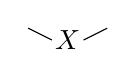
\begin{tikzpicture}[baseline=(a0.base), inner sep=1pt]
      \node (a0) {$X$};
      \draw (a0.west) -- ++(-.3,.15);
      \draw (a0.east) -- ++(.3,.15);
   \end{tikzpicture}
\end{walign}
The squared norms are quadratic, so delete-the-node handles them directly
($X$ appears twice in $\Tr(X^T X)$, giving the factor $2$).
The unsquared (129) and its Jacobian (130) compose the scalar function $\sqrt{\cdot}$
with a quadratic network --- exactly the chain-rule machinery of
Chapter~\ref{chapter:functions}.

\section{Derivatives of Structured Matrices}

So far $X$ had no special structure: every entry was a free parameter.
If $X$ is constrained --- symmetric, diagonal, Toeplitz ---
the free parameters are fewer, and the honest way to differentiate is to
write $X$ as a linear function of its free parameters and use the chain rule.
Diagrammatically, the constraint is one more tensor in the network:
the \emph{structure tensor} $S$ with
$X = S(\theta)$ for parameter vector (or matrix) $\theta$,
and the gradient with respect to $\theta$ is the unconstrained gradient
$G = \partial f/\partial X$ pushed through $S$.

\paragraph{Symmetric.}
For symmetric $X$ the independent parameters are the entries on and below the
diagonal, and pushing $G$ through the structure gives
\begin{walign}
   \tag{138}
   \frac{df}{dX}
   &= G + G^T - G \circ I
   \\
   \tag{139}
   \frac{\partial \Tr(AX)}{\partial X}
   &= A + A^T - A \circ I
   \\
   \tag{140}
   \frac{\partial \det(X)}{\partial X}
   &= \det(X)\big(2X^{-1} - X^{-1} \circ I\big)
   \\
   \tag{141}
   \frac{\partial \ln \det(X)}{\partial X}
   &= 2X^{-1} - X^{-1} \circ I
\end{walign}
The pattern $G + G^T$ is (twice) the symmetrization squiggle from the
introduction; the correction $G \circ I$ removes the double-counted diagonal,
drawn with copy tensors as
\[
   G \circ I \;=\;
   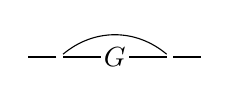
\begin{tikzpicture}[baseline=-.25em, inner sep=1pt]
      \node (d1) at (0,0) {$\sbullet$};
      \node (G) at (.7,0) {$G$};
      \node (d2) at (1.4,0) {$\sbullet$};
      \draw (d1) -- (G) -- (d2);
      \draw (d1) edge[bend left=40] (d2);
      \draw (d1) -- ++(-.4,0);
      \draw (d2) -- ++(.4,0);
   \end{tikzpicture}
\]
(the arc between the two copy tensors forces the row and column index to agree,
so only the diagonal of $G$ survives).
Note that (140) and (141) are just (49) and (57) pushed through the rule (138).

\paragraph{Diagonal.}
For diagonal $X = \diag(\theta)$ the structure tensor \emph{is} the order-3 copy
tensor, and the chain rule contracts $G$ with it:
\begin{walign}
   \tag{142}
   \frac{\partial \Tr(AX)}{\partial X}
   &= A \circ I
\end{walign}

\paragraph{Toeplitz.}
A Toeplitz matrix is constant along diagonals, one parameter per diagonal;
the gradient with respect to the $k$-th parameter is the sum of $G$ along the
$k$-th diagonal (see the exercises).

\section{Exercises}

\begin{exercise}
Derive (126) with diagrams:
draw $\Tr[(X^T C X)^{-1} (X^T B X)]$ as a closed chain containing four copies of
$X$ and one inverse node, apply delete-the-node to the two outer copies and the
splitting rule to the two inner ones, and collect terms using the symmetry of
$B$ and $C$.
\end{exercise}

\begin{exercise}
Prove $\frac{\partial \det(X^{-1})}{\partial X} = -\det(X^{-1})(X^{-1})^T$ (62)
by combining the determinant stack with the splitting rule.
\end{exercise}

\begin{exercise}
Prove the cofactor identity
$\sum_k \frac{\partial \det(X)}{\partial X_{ik}} X_{jk} = \delta_{ij} \det(X)$ (47)
by reinserting a copy of $X$ into the empty slot of the adjugate diagram.
% Hint: attaching X's column edge to the gap's column stub re-creates the
% closed stack whenever i = j; for i != j antisymmetry kills the diagram.
\end{exercise}

\begin{exercise}
Prove (58), $\partial \det(X^k)/\partial X = k \det(X^k) X^{-T}$:
the stack for $\det(X^k)$ contains $kn$ copies of $X$; deleting one and using
$\operatorname{adj}$ gives the result.
\end{exercise}

\begin{exercise}
Let $T$ be Toeplitz with parameters $t_{-n+1}, \dots, t_{n-1}$, one per diagonal.
Show that
$\frac{\partial \Tr(A^T T)}{\partial t_k}$ is the sum of the entries of $A$
along the $k$-th diagonal, and draw the structure tensor of $T$.
\end{exercise}

\begin{exercise}
Find the derivative of the Gaussian density
\[
   f(x,\Sigma,\mu) = \frac{1}{\sqrt{(2\pi)^k|\Sigma|}}
   \exp\left(-\frac12(x-\mu)^T \Sigma^{-1} (x-\mu)\right)
\]
with respect to $\Sigma$, combining the splitting rule, the log-determinant (57),
and the chain rule of Chapter~\ref{chapter:functions}.
% Answer: f * ( -1/2 Sigma^{-1} + 1/2 Sigma^{-1}(x-mu)(x-mu)^T Sigma^{-1} ),
% assuming symmetric Sigma without the structured correction; with (138) apply
% G + G^T - G o I to taste.
\end{exercise}
